\begin{equation}
    \begin{gathered}
        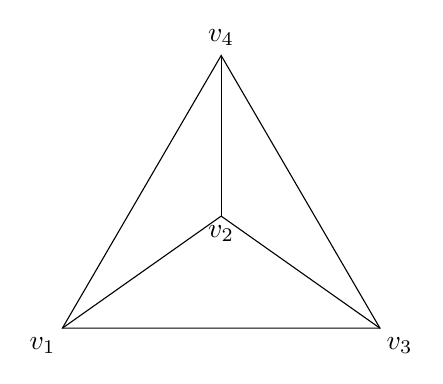
\begin{tikzpicture}[x=0.75pt,y=0.75pt,yscale=-1,xscale=1]
            %uncomment if require: \path (0,300); %set diagram left start at 0, and has height of 300
            
            %Shape: Triangle [id:dp7098951064257721] 
            \draw   (176.51,109) -- (253.02,240.38) -- (100,240.38) -- cycle ;
            %Straight Lines [id:da8162486890668672] 
            \draw    (176.51,109) -- (176.51,186.38) ;
            %Straight Lines [id:da2843979428920951] 
            \draw    (176.51,186.38) -- (100,240.38) ;
            %Straight Lines [id:da2477682584878509] 
            \draw    (253.02,240.38) -- (176.51,186.38) ;
            
            % Text Node
            \draw (98,243.78) node [anchor=north east] [inner sep=0.75pt]    {$v_{1}$};
            % Text Node
            \draw (176.51,189.78) node [anchor=north] [inner sep=0.75pt]    {$v_{2}$};
            % Text Node
            \draw (255.02,243.78) node [anchor=north west][inner sep=0.75pt]    {$v_{3}$};
            % Text Node
            \draw (176.51,105.6) node [anchor=south] [inner sep=0.75pt]    {$v_{4}$};
            \end{tikzpicture}                
    \end{gathered}.
    \label{eq:subgraph}
\end{equation}